\chapter{Introduction}\label{sec:introduction}
\graphicspath{{graphics/}{graphics/systems/}}

%\section{Motivation}

\section{Context}
\label{sec:context}
%\textit{Write something about project} \textsc{skye}\textit{, focus projects, ETH and/or ASL, DRZ. Motivation..} 

Within the Bachelor's course in mechanical engineering at the ETH Zurich it is offered to join a focus project instead of focus lectures. A focus project is often a novel or experimental design of a prototype\footnote{Some former projects can be found at \url{http://www.asl.ethz.ch/education/bachelor/focus}.} and elaborated over a period of two semesters within a team of mainly students in mechanical engineering, but often in cooperation with students from interdisciplinary courses. The project is settled at the Autonomous Systems Lab (ASL) at ETH Zurich in cooperation with Disney Research Zurich (DRZ). \\
Project \textsc{Skye} then was a focus project started in autumn \num{2011} and will be continued even after the ``official'' end of the project in summer 2012. The \textit{Rollout} event in the historic main building of ETH Zurich was a unique moment when the prototype wafted over the overwhelmed spectators. \\

\begin{figure}[H]
	\centering
    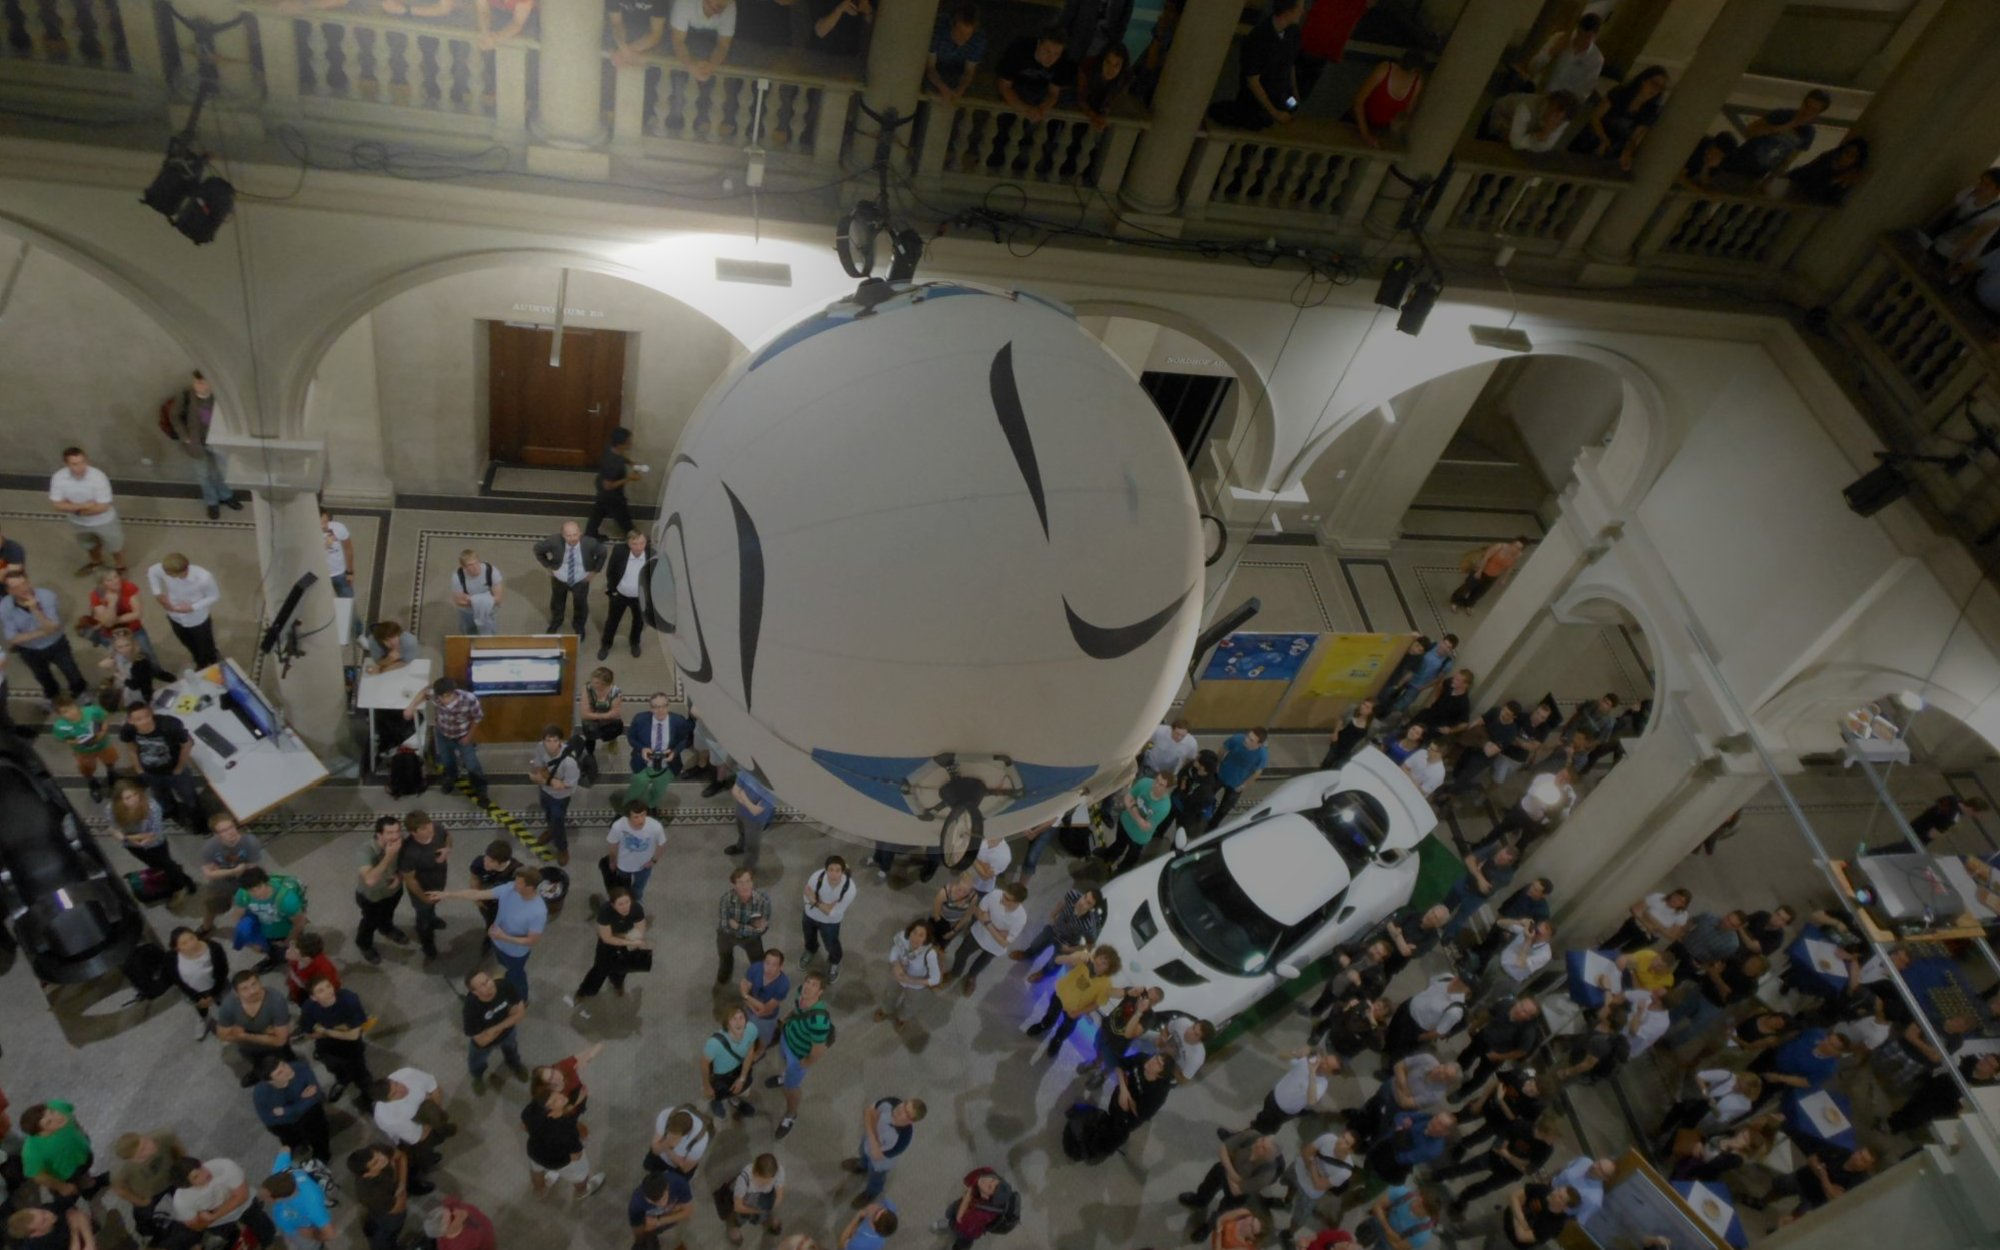
\includegraphics[width = 0.9\textwidth]{graphics/rollout2.jpg}
  \caption{The highligth of project \textit{Skye}: The \textit{Rollout} event on May 25, 2012 in the main hall of ETH Zurich.}
  \label{fig:rollout}
\end{figure}


\section{System Overview}
\label{sec:system overview}
%\textit{Description of \textsc{Skye}. Application fields, technical description, equipment, realization..} \\
\textsc{Skye} is a high agile unmanned aerial vehicle in form of a spherical blimp. It was developed to achieve a system for image capturing for 3D reconstruction as well as obtain entertainment functions (as airshows, human interaction etc.). As there exist already systems that fullfil these requirements\footnote{Mainly quadrotors, but also other UAV.} it was claimed to build a system that provides increased flight time and higher operating safety. \textsc{Skye} is the system that accomplishes these improvements. \\
The two-layered spheric hull is filled with lighter-than-air gas helium. The gas is filled in with an overpressure of \SI{15}{\milli\bar} that ensures a stiff hull surface without the need of any rigid structure. Four identical motor units are placed tetrahedrally on the hull by Velcro. The \textit{AHM 23-10 EPP 1045} thrusters are pointing tangential to the sphere. Their orientation can be rotated around the radial axis using a \textit{\textsc{Maxon} A-Max 16} motor. The center of gravity is approximately identical with the center of buoyancy. Further on, the gravitational force exceeds the buoyancy only for a minimum\footnote{So the system sinks slowly to ground if turned off.}.
\begin{figure}[H]
    \centering
    \def\svgwidth{0.8\columnwidth}
    \input{graphics/skye_description.pdf_tex}
    \caption{CAD sketch of \textsc{Skye}. Red arrows indicate thrust and orientation of the motor units. Blue tetrahedron indicates symmetrical arrangement of them. }
    \label{fig:scene_trajectoryFollowing}
\end{figure}
Further on, a camera system consisting on two light weighted \textit{Bluefox} cameras as well as a high end \textit{Prosilica} high resolution camera connected to a onboard \textit{Intel Atom} embedded computer are detached on the hull. The computer runs a Linux distribution and can be linked to via a Wi-Fi module. A low level \textit{Cortex M4} processor within a \textit{PX4FMU} Inertial Measurement Unit (IMU) controls the flight system. It is equipped with barometer, gyroscope, magnetometer, accelerometer and a GPS receiver. The control communication is realized with both a \textit{Lairtech Xbee} module and a \textit{Futaba Rasst 2.4GHz} receiver. \\
The high symmetrical system properties combined with the 8DOF actuation enable to fully control the holonomic 6DOF space. The 2 additional DOF are used for optimization (see \cite{schaffnervu}).  \\
Finally, the system is only as good as the user appreciates it. Therefore a optimal Human-Machine Interface (HMI) inevitable to provide a useful system. The aim of this thesis is to realize such a HMI in an optimal way for project \textsc{Skye}.
\section{Goals}
\label{sec:goals}
%\textit{Goals of this thesis:
%\begin{itemize}
%\item Define control modes
%\item Develop and realize HMI
%\item Trajectory generating
%\item Trajectory control
%\end{itemize}
%fun.. \\
%}
For this Bachelor's Thesis, intuitive interfaces to control and observe the system \textsc{Skye} had to be developed. This includes the implementation of a Graphical User Interface (GUI) for a computer based Ground Station (GS) based on any existing solution. Further on, different manual control modes and suitable Human-Machine Interfaces must have been elaborated and implemented. Finally, automatic manoeuvres  (paths and trajectories) had to be generated considering simplified dynamic system constraints based on the results from a model elaborated in \cite{weichart}. These goals are summarized in table \ref{tab:goals}. \\
\textbf{
Further on, the successful completion of project \textsc{Skye} could only be realized by invest a lot of effort for the compatibility of all system's part. Especially the integration of an alpha version IMU required thousands of tests to reach a full working system. bla bla Version Control, bla bla, das Zeugs gehoert wohl eher in die Conclusion..} So move it there;-)


\begin{table}[H]
\begin{center}
 \begin{tabular}{ll}
 \hline
 Goal & Specification  \\ \hline \hline
 Control Modes 	& 	Intuitive Control for Manual for 6DOF Blimp \\
 HMI			&	Suitable for Control Modes \\
 GUI         	& 	Provide System Info, Adapt Properties \\
 Trajectories   & 	Automatic Maneuvers \\
 \hline
 \end{tabular}
 \caption{Main goals of this thesis}\vspace{1ex}
 \label{tab:goals}
\end{center}
\end{table}


\section{Similar Systems and their HMI}
\label{sec:similar systems}
%\textit{About degrees of freedom, (non-)holonomic system control, car wheels, rezeros qgo sphere cite \cite{kammermann}.} \\
The HMI (or control device) for a machine mainly depends on its number of control inputs and its level of automation. To control more control inputs, additional sticks or motions have to be provided. Automation of the system can simplify its control, but requests for emergency backups in case of automation fail. \\
The number of control inputs depends on the systems possibilities. This is shown in table \ref{tab:systems_hmi}\footnote{\textsc{AMZ} racing: \url{http://www.amz.ethz.ch/} \\ \textsc{Rezero}: \url{http://rezero.ethz.ch/} \\ \textsc{Arac}: \url{http://www.arac.ethz.ch/} \\ \textsc{arDrone}: \url{http://ardrone2.parrot.com/}}. A car has 3DOF, i.e. it can move in a plane and turn around its yaw axis. But the driver cannot steer all those motions independently as no lateral motion is possible without longitudinal movements (the system has a nonholonomic constraint). So a steering wheel in combination with a gas and break pedal serve as HMI. For a ballbot or a legged robot each of the 3DOF can be steered directly (they are holonomic systems). Therefore the HMI device must enable three inputs as it is provided for instance by a Qgo Sphere\footnote{See \cite{kammermann}, section \ref{sub:hardware} or \url{http://www.quasmo.ch/index.php/qgosphere} for more informations about Qgo Sphere.} or a gamepad. A quadrotor is comparable to the system \textsc{Skye}. A quadrotor is a nonholonomic system, as roll and pitch angle are coupled with the lateral and longitudinal motion. Therefore out of the 6DOF in space, only 4 can be controlled independently by the pilot. A gamepad or even a smartphone are suitable control devices. As \textsc{Skye} is (due to its mechanics and actuation symmetry) a holonomic system, all the 6DOF can be steered individually. This requires a HMI with even more control inputs.
%In a car, the driver controls the steer angle and the acceleration. Although this is not sufficient to move the car into any desired direction\footnote{As the lateral motion depends on the turning angle, the system is nonholonomic.} the steering wheel and gas pedal provide sufficient and intuitive control to drive from a to b. The pilot of an airplane can move through the three dimensional space and has therefore more freedom to control its vehicle than the car driver. As a drawback, he has to consider even more control inputs (joystick for pitch and roll, rudder pedals for yaw and throttle control for thrust). As the system dynamics of \textsc{Skye} only depend on holonomic constraints, its motion in the 3D space can be controlled for every of the 6DOF independently. As a drawback, the pilot would have to consider 6 control inputs at the same time. The elaboration of finding a suitable solution for the piloting of \textsc{Skye} is described in chapters \ref{cha:DifferentControlModes} and \ref{cha:findHardSoftSolution}.

\begin{table}[H]
\begin{center}
\newcolumntype{M}{>{$\vcenter\bgroup\hbox\bgroup}c<{\egroup\egroup$}} 
 \begin{tabular}{MMMMM}
 \hline
 System & DOF & Non\-holonomic & Inputs & Device \\ 
  \hline \hline 
     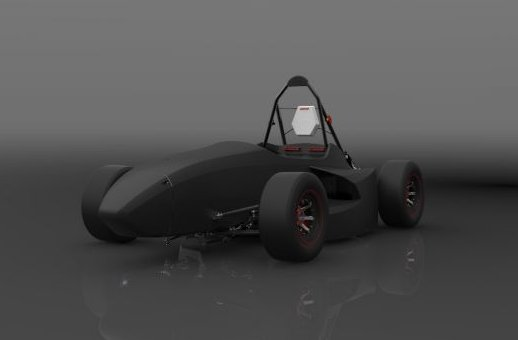
\includegraphics[width = 0.25\textwidth]{amz.jpg}
   & 	3 & 1  & 2 & 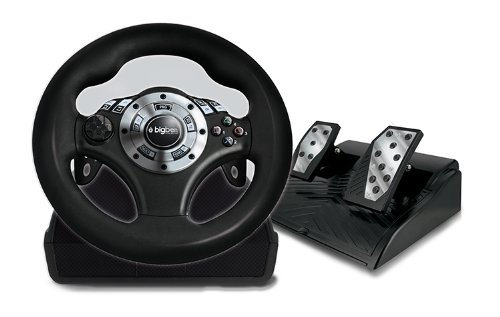
\includegraphics[width = 0.18\textwidth]{steeringwheel.jpg} \\
  \hline
    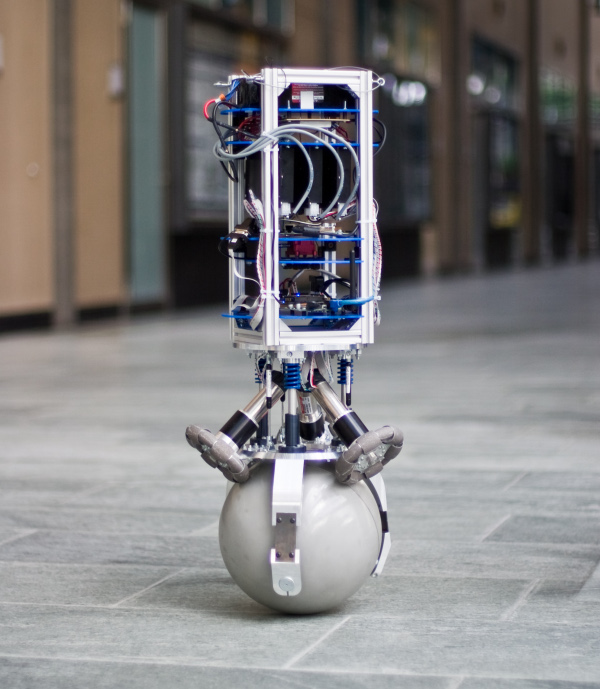
\includegraphics[width = 0.25\textwidth]{rezero.jpg}
   & 	3 & 0  & 3 & 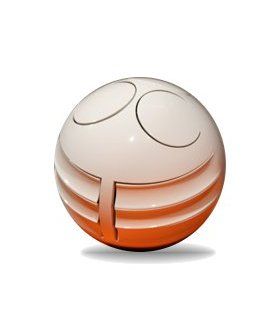
\includegraphics[width = 0.18\textwidth]{HMI/qgo_sphere_cut.jpg} \\
  \hline
    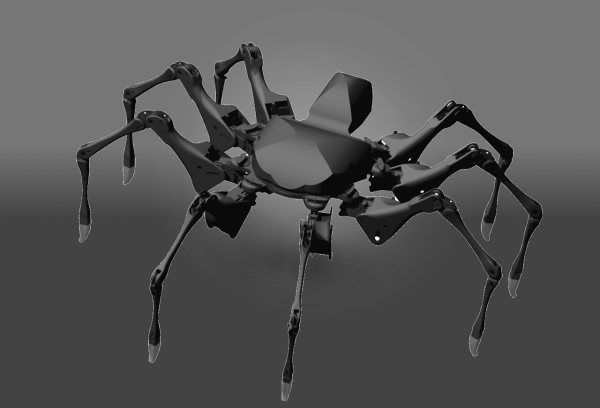
\includegraphics[width = 0.25\textwidth]{arac.jpg}
   & 	3 & 0  & 3 & 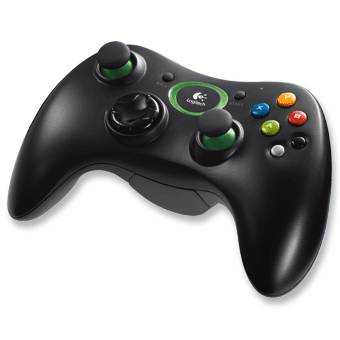
\includegraphics[width = 0.14\textwidth]{gamepad.jpg} \\
  \hline
    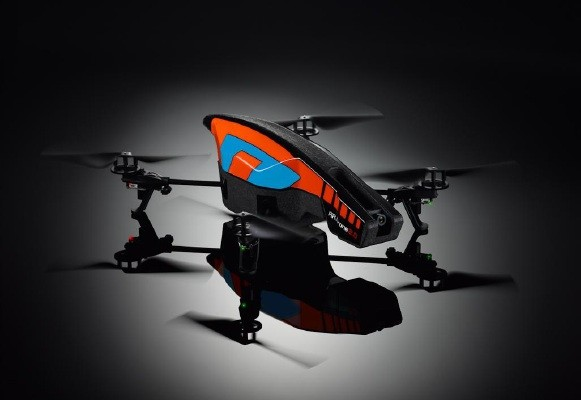
\includegraphics[width = 0.25\textwidth]{ardrone.jpg}
   & 	6 & 2  & 4 & 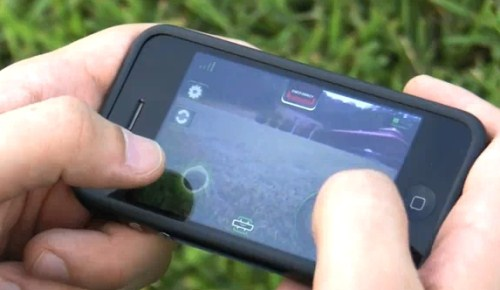
\includegraphics[width = 0.18\textwidth]{iphone.jpg} \\
  \hline
    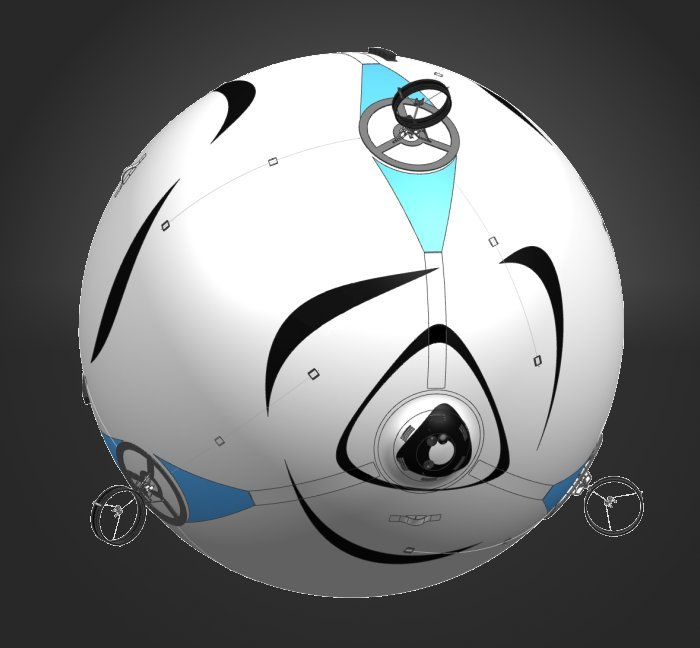
\includegraphics[width = 0.25\textwidth]{skye.jpg}
   & 	6 & 0  & 6 & 
\includegraphics[width = 0.1\textwidth]{questionmark.eps} \\
 \hline
 \end{tabular}
 \caption{Some examples of systems and their HMI. The number of inputs depends on the number of degree of motion reduced by nonholonomic constraints.}\vspace{1ex}
 \label{tab:systems_hmi}
\end{center}
\end{table}


\section{Structure of the Report}
\label{structure}
%\textit{First about HMI, then about trajectories.. \\ results are shown within the corresponding chapter and in the appendix. Discussion/Conclusion in the end of the report.} \\
This report is divided into two parts. The first part including chapter \ref{cha:DifferentControlModes} and \ref{cha:findHardSoftSolution} treats the problem described above to find a suitable solution to steer \textsc{Skye}. First, the different elaborated control modes are shown in chapter \ref{cha:DifferentControlModes}. The following chapter \ref{cha:findHardSoftSolution} contains the evaluation of different control devices and describes the realized HMI. Especially the GUI is described in detail in section \ref{subsec:qGroundControl}. \\ The second part of this thesis is a more technical elaboration of optimal trajectory generation for the system \textsc{Skye} (chapter \ref{cha:trajectory}). Some of the trajectory control results are shown as well in this chapter. Further results are found in the appendix.